\chapter{The Hello World example}
\epigraph{\textit{``It's a dangerous business, Frodo, going out of your door,'' he used to say. ``You step into the Road, and if you don't keep your feet, there is no knowing where you might be swept off to.''}}{J.R.R. Tolkien, \textit{The Fellowship of the Ring} (1954)}



\MakeShortVerb{\!} % makes \verb|foo| == !foo!

As well as defining a wire protocol for information exchange in different marshalling schemes, Goby provides a number of useful classes and applications that are written in C++.  We feel that C++ is a good blend of elegance, speed, and expressiveness, and we hope that you will come to agree. For next few chapters we will cover these tools. If you are eager to learn about the Goby wire protocol or wish to use Goby with another programming language, please refer to Chapter \ref{chap:underpinnings}.

While the core of Goby is based on a number of advanced C++ techniques, you only need a small amount of C++ knowledge to get started writing your own Goby application. If you are new to programming and C++, we recommend Prata's \textit{C++ Primer Plus} \cite{Prata:2001:CPP:515923}. If you are experienced in programming but new to C++, we recommend Stroustrup's \textit{The C++ Programming Language} \cite{Stroustrup:2000:CPL:518791}. The website \url{www.cplusplus.com} is an excellent online reference.

This complete example is located at the end of this chapter in section \ref{sec:hello_example_code}. It's probably a good idea to download and install Goby now so you can try this out for yourself: \url{https://launchpad.net/goby}. There's really no substitute for trying (and breaking) things yourself.

This example involves passing a single type of message (class HelloWorldMsg) from one Goby application (!hello_world1_g!\footnote{you can name your applications whatever you want, but we like appending ``\_g'' to the end to indicate that this is a Goby application.}) to another (!hello_world2_g!).  See Fig. \ref{fig:hello_world_sketch} for a sketch of the components in this example. Since the default configuration for Goby uses \gls{multicast} communications, there is no \gls{daemon} or server to concern ourselves with. A good analogy to this multicast group is a meeting amongst peers. Everyone is in the same room, but no one explicitly controls the conversation. People tune in (!subscribe!) for topics (messages) that interest them and ignore those that do not.

!hello_world1_g! and !hello_world2_g! reside on the same \gls{platform}, which for now we will assume is the same computer. We will learn about inter-platform communication later on.

\begin{figure}
\centering
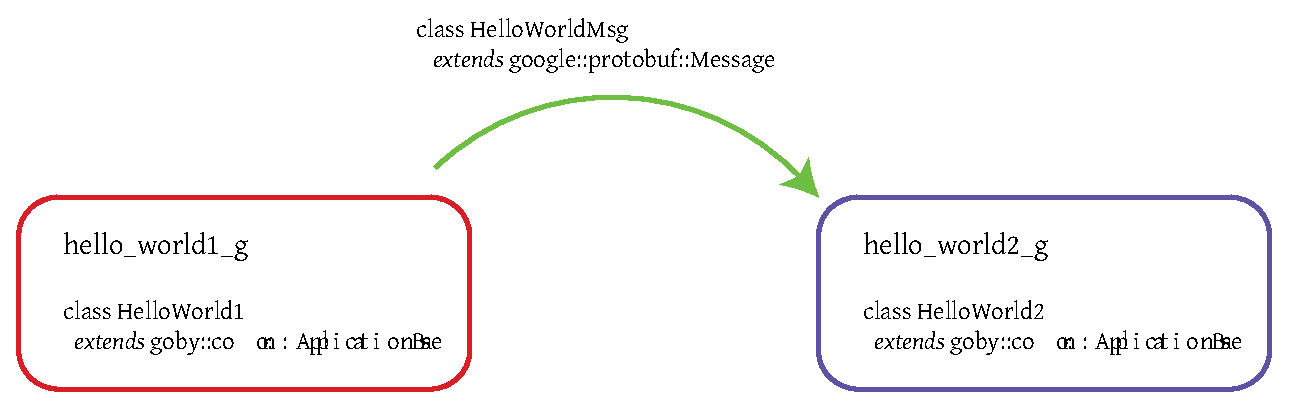
\includegraphics[width=\textwidth]{hello_world_sketch}
\caption{In this example \texttt{hello\_world1\_g} publishes messages of type \texttt{HelloWorldMsg} to the subscriber \texttt{hello\_world2\_g}.}
\label{fig:hello_world_sketch}
\end{figure}

\section{Meeting goby::core::ApplicationBase}

!goby::core::ApplicationBase! is the building block (\gls{base class}) upon which we will make our Goby applications (which will be \glspl{derived class} of ApplicationBase). !ApplicationBase! provides us with a number of tools; the main ones are:

\begin{itemize}
\item a constructor !ApplicationBase()! that reads the command line parameters and the configuration file (we will learn about this in Chapter \ref{chap:gps_driver}) and connects to the \gls{multicast} group for us.
\item a virtual method !loop()! that is called at a regular frequency (10 Hertz by default).
\item a method !subscribe()! which tells !gobyd! that we wish to receive all messages of this type.
\item a method !newest()! which returns the newest (latest received) message of a given type that we have previously called !subscribe()! for. We will learn how to filter the subscriptions later.
\item a method !publish()! allowing us to publish messages to the multicast group and thereby to any subscribers of that type.
\item an object !goby::glog! which acts just like std::cout and lets us write to our choice of debug logs (terminal window / text file) with fine grained control over the verbosity of the output.
\end{itemize}

\section{Creating a simple Google Protocol Buffers Message: HelloWorldMsg}\label{sec:proto_ex}

\glsreset{protobuf} \gls{protobuf} allows us to create custom messages for holding and transmitting data in a structured (object-based) fashion. These protobuf messages are similar to data structures (!struct!s) available in many languages. Transmitting data typically is done in a long string of bytes. However, humans do not view the world as a string of bytes. We think and communicate using tangible and intangible objects. For example, a ball might be described by its diameter, color, and weight. A message describing a baseball might be written in protobuf as such:
\begin{boxedverbatim}
// ball.proto
message Ball
{
   required double diameter = 1;
   enum Color { WHITE = 1; BLACK = 2; SPOTTED = 3 }
   optional Color color = 2;
   optional double weight = 3;
}
\end{boxedverbatim}
\resetbvlinenumber
We will learn the meaning of !required!, !optional! and the sequence numbers (!=1!, !=2!, etc.) shortly.

Similarly, a sample from a CTD\footnote{Conductivity-Temperature-Depth} sensor can be thought of as an object containing a number of floating point values representing salinity, temperature, pressure, etc. In the \gls{protobuf} language:
\begin{boxedverbatim}
import "units_extensions.proto"
// ctd_sample.proto
message CTDSample
{
   required double salinity = 1 [(units)="none"];
   required double temperature = 2 [(units)="degC"];
   required double depth = 3 [(units)="m"];
}
\end{boxedverbatim}
\resetbvlinenumber
Goby (using protobuf objects) allows messages to be formed using this more natural object-based representation.

As you may have noticed from these examples, the \gls{protobuf} language is simple with a syntax similar to that of C. Protobuf messages are written in .proto files and passed to the protobuf compiler (!protoc!) which generates C++ code to pass to the C++ compiler (!c++!, !gcc! on Linux). See Fig. \ref{fig:hello_world_compile} for a graphical representation of this compilation process. 

\begin{figure}
\centering
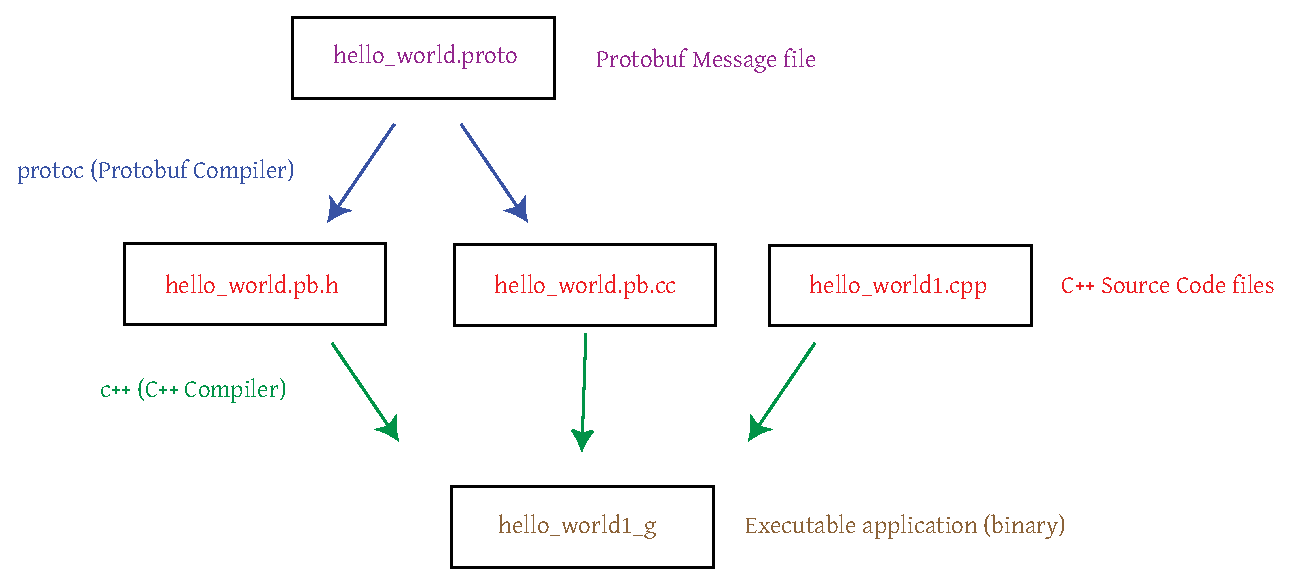
\includegraphics[width=\textwidth]{hello_world_compile}
\caption{The steps of compiling \texttt{hello\_world1\_g.} We write the files \texttt{hello\_world.proto} and \texttt{hello\_world1.cpp} and the rest are generated by tools (\texttt{protoc} and \texttt{c++}.}
\label{fig:hello_world_compile}
\end{figure}

Protobuf messages can contain a number of basic types (or vectors of these types) as well as nested messages. Fields are labeled as required, optional or repeated (essentially a vector). Required fields must be filled in; clearly, optional fields can be omitted. This might be a good time to read the excellent Protocol Buffers tutorial \cite{proto-tutorial} to get a feel for the language and usage.

As you become familiar with using \gls{protobuf}, the language reference \cite{proto-lang-ref} will help you in creating .proto files and the generated code reference \cite{proto-gen-code} will assist you in accessing the C++ classes created by the !.proto! files when passed through !protoc!.

For this example, we wish to send ``hello world'' (of course) so we need a string to hold our message that we will call `telegram': 
\begin{verbatim}
required string telegram = 1;
\end{verbatim}
The ! = 1! simply indicates that `telegram' is the first field in the message !HelloWorldMsg!. Furthermore, we want to keep track of how many times we've said ``hello'' so we'll add an unsigned integer called `count'
\begin{verbatim}required uint32 count = 2;\end{verbatim}
The resulting .proto file is given in section \ref{sec:hello_world.proto}.

We chose `required' to prefix both fields because we feel that a valid !HelloWorldMsg! must contain both a `telegram' and a `count.' !uint32! is an unsigned (non-negative) 32 bit integer. The numbers following the ``='' sign are unique identifiers for each field. These numbers can be chosen however one likes as long as they are unique within a given protobuf message. Ascending numbers in the order fields are declared in the file is a reasonable choice.

This .proto file is ``compiled'' into a class with the same name as the message (!HelloWorldMsg!). This class is accessed by including a header file with the same name as the .proto file, but with ``.proto'' replaced with ``.pb.h''. Furthermore, we can set the contents of this class using calls (``mutators'' or ``setters'') that are the same as the field name (i.e. `telegram' or `count') prepended with ``set\_'':
\begin{boxedverbatim}
// C++ 
#include "hello_world.pb.h"

// create and populate a ``HelloWorldMsg'' called `msg'
HelloWorldMsg msg;
msg.set_telegram("hello world");
msg.set_count(3);
\end{boxedverbatim}
\resetbvlinenumber

and access them using these methods (``accessors'' or ``getters'') that have the same function name as the field name:

\begin{boxedverbatim}
// C++ 
// print information about `msg' to the screen
std::cout << msg.telegram() << ": " << msg.count() << std::endl;
\end{boxedverbatim}
\resetbvlinenumber


\section{Learning how to \textit{publish}: HelloWorld1}

To create a Goby application, one needs to

\begin{itemize}
\item create a derived class of !goby::core::ApplicationBase!. We also must include the goby core header (!#include "goby/core.h"!).
\item create an overloaded !loop()! method (which can do nothing).
\item run the application using the !goby::run()! function. Because goby::core::ApplicationBase reads our configuration (including command line options) for us, we also pass !argv! and !argc! to !run()!.
\end{itemize}

That is all one needs to create a valid working Goby application. All together the ``bare-bones'' Goby application looks like:

\begin{boxedverbatim}
#include "goby/core.h"

class DoNothingApplication : public goby::core::ApplicationBase 
{
  void loop() {}
};

int main(int argc, char* argv[])
{   
    return goby::run<DoNothingApplication>(argc, argv);
}
\end{boxedverbatim}
\resetbvlinenumber

However, we would like our application to do a little bit more.

ApplicationBase provides a pure \gls{virtual} method called !loop()! that is called on some regular interval (it is the \textit{\gls{synchronous} event} in Goby), by default 10 Hertz. By overloading !loop()! in our derived class !HelloWorld1!, we can do any kind of synchronous work that needs to be done without tying up the CPU all the time\footnote{in between calls to \texttt{loop()}, ApplicationBase handles incoming subscribed messages}. In this example, we will create a simple message (of type !HelloWorldMsg! which we previously designed in section \ref{sec:proto_ex}) and publish it to all subscribers (we create a subscriber in section \ref{sec:sub_ex}). 

Let's walk through each line of our !loop()! method:

\begin{boxedverbatim}
void loop()
{
   static int i = 0;
   HelloWorldMsg msg;
   msg.set_telegram("hello world!");
   msg.set_count(++i);
   goby::glog << "sending: " << msg << std::endl;
   publish(msg);
}
\end{boxedverbatim}
\resetbvlinenumber

\begin{itemize}
\item Line !1!: !loop()! takes no arguments and returns nothing (void). 
\item Line !3!: We declare a static integer\footnote{static in this context means that the variable will keep its value across calls to the function \texttt{loop()}.} to keep track of how many times we have looped and thus print an increasing integer value. 
\item Line !4!: We create an instantiation of !HelloWorldMsg! called !msg!.
\item Line !5!: We set the `telegram` field of the !HelloWorldMsg! named !msg!
\item Line !6!: We set the `count` field of !msg! and increment !i!.
\item Line !7!: We publish a human debugging log message using !goby::glog! (just like std::cout or other std::ostreams), which will be put to the terminal window in verbose mode\footnote{goby provides operator<< for google::protobuf::Message objects as a wrapper for google::protobuf::Message::DebugString()}. 
\item Line !8!: Finally, we publish our message. The entirety of the code for !hello_world1_g! is listed in section \ref{sec:hello_world1.cpp}.
\end{itemize}

\section{Learning how to \textit{subscribe}: HelloWorld2} \label{sec:sub_ex}

Now that our !hello_world1_g! application is publishing a message, we would like to create an application that subscribes for it. To subscribe for a message, we typically provide two things:
\begin{itemize}
\item The type of the message we want to subscribe for (e.g. !HelloWorldMsg!).
\item A method or function that should be called when we receive a message of that type (a callback).
\end{itemize}

Subscriptions typically take place in the constructor (here, !HelloWorld2::HelloWorld2()!), but can happen at any time as needed (within !loop()!, for example). You subscribe for a type once, and then you will continue to receive all other applications' publishes to that type.

We subscribe for a type using a call to !subscribe()! that looks like this:
\begin{boxedverbatim}
subscribe<HelloWorldMsg>(&HelloWorld2::receive_msg, this);
\end{boxedverbatim}
\resetbvlinenumber

While a bit complicated at first, this call should make sense shortly. It reads ``!subscribe! for all messages of type !HelloWorldMsg! and when you receive one, call the method !HelloWorld2::receive_msg! which is a member of !this! class (!HelloWorld2!).''\footnote{You can call a member function (method) of another class by passing the pointer to the desired class instantiation instead of \texttt{this}. Alternatively, you can call a non-class function by just giving its pointer, e.g. \texttt{subscribe(\&receive\_msg)}.}. The method provided as a callback (here !receive_msg()!) must have the signature
\begin{boxedverbatim}
void func(const ProtoBufMessage&); 
\end{boxedverbatim}
\resetbvlinenumber
where !ProtoBufMessage! is the type subscribed for (here, !HelloWorldMsg!). !receive_msg()! has that signature
\begin{boxedverbatim}
void HelloWorld2::receive_msg(const HelloWorldMsg& msg);
\end{boxedverbatim}
\resetbvlinenumber
and thus is a valid callback for this subscription. After subscribing, !receive_msg()! will be called immediately (an \gls{asynchronous} event) upon receipt of a message of type !HelloWorldMsg! unless
\begin{itemize}
\item !loop()! is in the process of being called or
\item another message callback (for another subscribed type) is in the process of being called.
\end{itemize}
In these cases, !receive_msg()! is called as soon as the blocking method returns. These conditions allow Goby applications to be single threaded. Parallelism is gained via multiple applications that communicate via messages, avoiding the extremely tricky task of data access control (using ugly things like mutexes, semaphores, etc.)

For this example, inside of !receive_msg()! we simply post the message to the debug log (!goby:glog!):

\begin{boxedverbatim}
void receive_msg(const HelloWorldMsg& msg)
{
   goby::glog << "received: " << msg << std::endl;
}
\end{boxedverbatim}
\resetbvlinenumber

The full source listing for !hello_world2_g! can be found in section \ref{sec:hello_world2.cpp}.

\section{Compiling our applications using CMake}

!CMake! \cite{cmake}, while still lacking in documentation, is probably the easiest way to build software these days, especially for cross platform support. I will briefly walk through building a Goby application using !CMake! within the larger Goby examples configuration (depending on how you installed Goby, !goby/share/examples! or !/usr/share/goby/examples!). If you look at the !CMakeLists.txt! file in \ref{sec:hello_world:CMakeLists.txt}, you can see the steps needed to add our new applications to the project:

\begin{boxedverbatim}
protobuf_generate_cpp(PROTO_SRCS PROTO_HDRS hello_world.proto)
add_executable(hello_world1_g hello_world1.cpp ${PROTO_SRCS} ${PROTO_HDRS})
target_link_libraries(hello_world1_g goby_pb)
\end{boxedverbatim}
\resetbvlinenumber

Line 1 tells !CMake! to add ``hello\_world.proto'' to the files needed to be pre-compiled by the Google Protocol Buffers compiler !protoc!. protobuf\_generate\_cpp is provided by the CMake module \href{http://bazaar.launchpad.net/~goby-dev/goby/trunk/annotate/head:/cmake_modules/FindProtobufGoby.cmake}{goby/cmake\_modules/FindProtobufGoby.cmake}. Line 2 adds our application !hello_world1_g! to the list to be compiled by the C++ compiler, using the sources !hello_world1.cpp! and the generated Protocol Buffers code. We append ``\_g'' as a convention to quickly recognize Goby applications. Line 3 links our application against the goby\_core library, which provides goby::core::ApplicationBase, our base class. The process of steps !CMake! is using to compile our code is illustrated in Fig. \ref{fig:hello_world_compile}.

Adding !hello_world2_g! is directly analogous.

\section{Trying it all out: running from the command line}

Now, assuming you've compiled everything, we can run the example.

You'll need two terminal windows, one for each of our ``hello world'' applications. Now we can launch our two applications (we can launch in either order but if we start the publisher !hello_world1_g! after the subscriber !hello_world2g!, we will miss the first few messages.). We add the ``-v'' flag to indicate we want verbose terminal output and the ``--no\_db'' flag to indicate that we aren't logging data to the !goby_database!. You can always use ``-h'' to get help on the command line parameters.

\begin{boxedverbatim}
> hello_world2_g -v --no_db
> hello_world1_g -v --no_db
\end{boxedverbatim}
\resetbvlinenumber

You should see !hello_world1_g! passing messages to !hello_world2_g! every 1/10th second.

\subsection{hello\_world1\_g output}
\begin{boxedverbatim}
hello_world1_g (20110421T123431.832807): (Warning): Not using
`goby_database`. You will want to ensure you are logging your 
runtime data somehow
hello_world1_g (20110421T123432.000169): sending: ### HelloWorldMsg ###
hello_world1_g (20110421T123432.000309): telegram: "hello world!"
hello_world1_g (20110421T123432.000382): count: 1
hello_world1_g (20110421T123432.000448): 
hello_world1_g (20110421T123432.099503): sending: ### HelloWorldMsg ###
hello_world1_g (20110421T123432.099638): telegram: "hello world!"
hello_world1_g (20110421T123432.099707): count: 2
hello_world1_g (20110421T123432.099770): 
hello_world1_g (20110421T123432.199695): sending: ### HelloWorldMsg ###
hello_world1_g (20110421T123432.199829): telegram: "hello world!"
hello_world1_g (20110421T123432.199898): count: 3
hello_world1_g (20110421T123432.199960): 
\end{boxedverbatim}
\resetbvlinenumber
The warning is emitted because of the ``--no\_db'' flag. That's ok for now.

\subsection{hello\_world2\_g output}
\begin{boxedverbatim}
hello_world2_g (20110421T123524.001344): received: ### HelloWorldMsg ###
hello_world2_g (20110421T123524.001899): telegram: "hello world!"
hello_world2_g (20110421T123524.001959): count: 1
hello_world2_g (20110421T123524.002012): 
hello_world2_g (20110421T123524.100828): received: ### HelloWorldMsg ###
hello_world2_g (20110421T123524.100916): telegram: "hello world!"
hello_world2_g (20110421T123524.100970): count: 2
hello_world2_g (20110421T123524.101021): 
hello_world2_g (20110421T123524.201065): received: ### HelloWorldMsg ###
hello_world2_g (20110421T123524.201161): telegram: "hello world!"
hello_world2_g (20110421T123524.201215): count: 3
hello_world2_g (20110421T123524.201264): 
\end{boxedverbatim}
\resetbvlinenumber


\section{Code} \label{sec:hello_example_code}

This entire example can be browsed online at \url{http://bazaar.launchpad.net/~goby-dev/goby/1.0/files/head:/share/examples/core/ex1_hello_world}.

\subsection{goby/share/examples/core/ex1\_hello\_world/hello\_world.proto} \label{sec:hello_world.proto}
\boxedverbatiminput{"@RELATIVE_CMAKE_SOURCE_DIR@/share/examples/core/ex1_hello_world/hello_world.proto"}
\resetbvlinenumber

\subsection{goby/share/examples/core/ex1\_hello\_world/hello\_world1.cpp}\label{sec:hello_world1.cpp}
\boxedverbatiminput{"@RELATIVE_CMAKE_SOURCE_DIR@/share/examples/core/ex1_hello_world/hello_world1.cpp"}
\resetbvlinenumber

\subsection{goby/share/examples/core/ex1\_hello\_world/hello\_world2.cpp}\label{sec:hello_world2.cpp}
\boxedverbatiminput{"@RELATIVE_CMAKE_SOURCE_DIR@/share/examples/core/ex1_hello_world/hello_world2.cpp"}
\resetbvlinenumber
\subsection{goby/share/examples/core/ex1\_hello\_world/CMakeLists.txt}\label{sec:hello_world:CMakeLists.txt}
\boxedverbatiminput{"@RELATIVE_CMAKE_SOURCE_DIR@/share/examples/core/ex1_hello_world/CMakeLists.txt"}
\resetbvlinenumber

\DeleteShortVerb{\!}
